% Inbuilt themes in beamer
\documentclass[aspectratio=169]{beamer}
\usepackage{graphicx}
\usepackage{amsmath}
% Theme choice:
\usetheme{CambridgeUS}

% Title page details: 
\title{Chapter 16: Monopolistic Competition} 
\author{Discussion section 4}
\date{December 2023}

\begin{document}

% Title page
\begin{frame}
    \titlepage 
\end{frame}

\begin{frame}{Outline}
Most markets are neither perfectly competitive nor monopolies.

\vspace{5mm}

Most will contain some elements of both:
\begin{itemize}
    \item Oligopolies (next chapter)
    \item Monopolistic competition (this chapter)
\end{itemize}
\end{frame}

\begin{frame}{Monopolistic competition}
    A monopolistically competitive market has:
    \begin{itemize}
        \item Many sellers
        \item Differentiated products
        \item Free entry an exit
        \item Similar production technologies
    \end{itemize}

    How does a monopolistically competitive firm choose its price?
\end{frame}

\begin{frame}{Price}
    \begin{itemize}
        \item Monopolistically competitive firm wants to maximize profits
        \item Does so by setting MR=MC
        \item This means P $>$ MC and there may be positive profits
    \end{itemize}

    Is this sustainable?
\end{frame}

\begin{frame}{Demand curve}
    \centering
    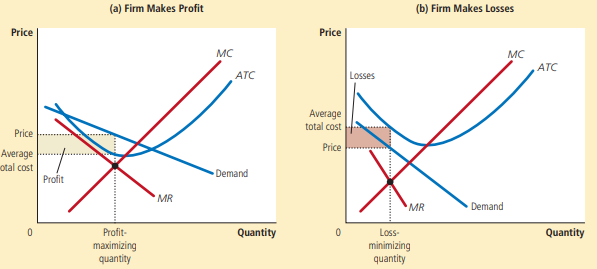
\includegraphics[width = 0.9\textwidth,keepaspectratio]{../figs/MCprofit.png}
\end{frame}

\begin{frame}{Entry/exit}
    \begin{itemize}
        \item Of course, non-zero profits cannot be sustained
        \item Negative profits lead to exit
        \item Positive profits lead to entry \textit{for substitute goods}
        \begin{itemize}
            \item What do we have to assume here?
        \end{itemize}
    \end{itemize}

    What does entry for substitute goods do to the profits of the monopolistically competitive firm?
\end{frame}

\begin{frame}{Entry}
    What does entry for substitute goods do to the profits of the monopolistically competitive firm?
    \begin{itemize}
        \item Introduction of substitute goods shifts the demand curve
        \item Process will continue until profits fall to 0
        \item When will this occur? Specifically, relationship between P, MC, and MR?
    \end{itemize}
    
\end{frame}

\begin{frame}{Profit-maximizing point}
    \begin{itemize}
        \item We know profits will be 0: this happens when P=ATC
        \item We know firms will maximize profits: this occurs when MR=MC
        \item Since maximum profits are 0, firm will choose Q such that MR=MC and P=ATC
    \end{itemize}
    Then we're ready to answer:
    \begin{enumerate}
        \item What characteristic of a monopoly does monopolistic competition have?
        \item What characteristic of perfect competition?
    \end{enumerate}
    
\end{frame}

\begin{frame}{Characteristics}
    What characteristic of a monopoly does this have? What characteristic of perfect competition?
    \begin{enumerate}
        \item Like a monopoly, P$>$MC
        \item Like a competitive market, P=ATC and profits are 0
        \item Q is lower than the efficient (perfectly competitive) level
    \end{enumerate}
\end{frame}

\begin{frame}{Demand curve}
    \centering
    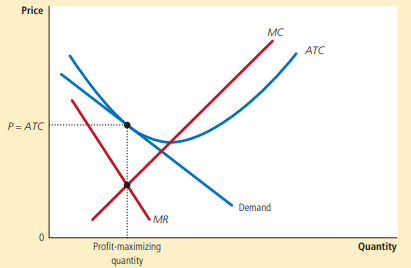
\includegraphics[width = 0.6\textwidth,keepaspectratio]{../figs/MCeq.png}
\end{frame}

\begin{frame}{Efficiency}
    \begin{itemize}
        \item The \textit{efficient production} minimizes ATC; not what happens here
        \item There is a \textit{markup} over the MC: some gap by which P $>$ MC.
        \begin{itemize}
            \item Does this mean there are positive profits?
        \end{itemize} 
        \item Is there deadweight loss? How do we know?
    \end{itemize}
\end{frame}

\begin{frame}{Efficiency}
    \begin{itemize}
        \item The \textit{efficient production} minimizes ATC; not what happens here
        \item There is a \textit{markup} over the MC: some gap by which P $>$ MC.
        \begin{itemize}
            \item Does this mean there are positive profits?
            \item No! Just means not at the efficient point.
        \end{itemize} 
        \item Is there deadweight loss? How do we know?
        \begin{itemize}
            \item Yes! There are consumers who value the good at greater than MC, would enjoy it in the free market, but can't buy in the monopolistically competitive market.
        \end{itemize}
    \end{itemize}
\end{frame}

\begin{frame}{Entry/exit}
    Monopolistic competition may exhibit an inefficient level of firm entry/exit.

    \vspace{5mm}

    What is the effect of firm entry?
\end{frame}

\begin{frame}{Entry/exit}
    What is the effect of firm entry?
    \begin{itemize}
        \item Since consumers have a taste for variety, there is a \textit{positive externality} to introducing new products: consumer surplus goes up
        \item Since new firms will decrease profits from existing firms who lose business, there is a negative externality on other firms
    \end{itemize}

    Net effect is ambiguous.
\end{frame}

\begin{frame}{Advertising}
    \begin{itemize}
        \item Does advertising exist in a perfectly competitive market?
        \item What is the impact of advertising?
        \item Is it good or bad for society?
    \end{itemize}
\end{frame}

\begin{frame}{Advertising}
    \begin{itemize}
        \item Does advertising exist in a perfectly competitive market?
        \begin{itemize}
            \item No! No point.
        \end{itemize}
        \item What is the impact of advertising?
        \begin{itemize}
            \item Informs consumers
            \item Or... \textit{misleads} consumers
        \end{itemize} 
        \item Is it good or bad for society?
        \begin{itemize}
            \item Don't know! Can't even say if it impedes or helps competition.
        \end{itemize}
    \end{itemize}
\end{frame}

\end{document}